
%A modo de introducción, comenzamos esta sección mostrando los datos demográficos obtenidos. Más adelante, continuamos con un análisis más exhaustivo de inteligibilidad y por separado se realizará otro análisis respecto a la nacionalidad atribuida a las oraciones. Por último para evaluar la hipótesis original, compondremos estos dos ejes para dilucidar el grado de validez de los resultados.

\section{Datos demográficos}

Se encuestaron $109$ participantes de los cuales se obtuvieron $352$ resultados. Como puede verse en la Figura \ref{genero} del total de participantes, $49$ pertenecían al rango comprendido entre $18$ y $25$ años, $43$ estaban en el rango $26$-$35$. $17$ de los participantes eran mayores a $35$ años.

\begin{figure}
\centering
\begin{subfigure}{.5\textwidth}
  \centering
	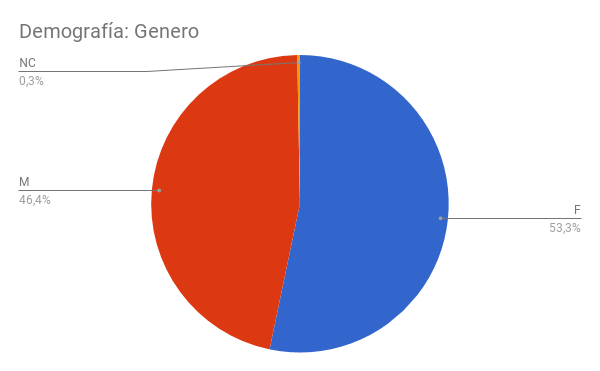
\includegraphics[trim={0 0 0 1.6cm},clip,width=1\linewidth]{datosDemograficos/genero.png}
  \caption{Distribución de géneros}
  \label{genero}
\end{subfigure}%
\begin{subfigure}{.5\textwidth}
  \centering
	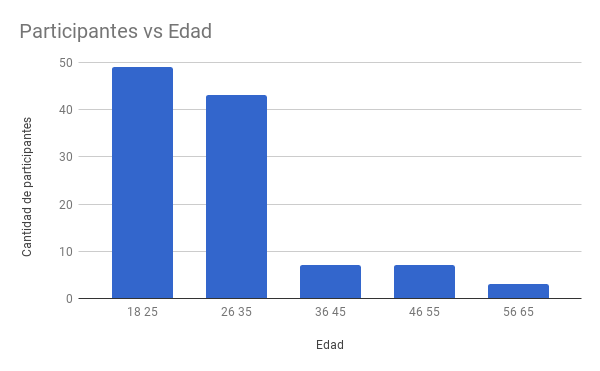
\includegraphics[trim={0 0 0 1.6cm},clip,width=1\linewidth]{datosDemograficos/edad.png}
  \caption{Cantidad de participantes por rango de edad}
  \label{fig:sub2}
\end{subfigure}
\caption{Datos demográficos de los participantes}
\label{edad}
\end{figure}

Con respecto al género de los participantes (Figura \ref{edad}), $187$ respuestas fueron brindadas por participantes del género femenino mientras que $163$ respuestas fueron brindadas por participante del género masculino .

Con respecto de la región en que cada participante pasó su infancia puede verse en la Figura \ref{distTerritorial} una predominancia de personas del Gran Buenos Aires con $45\%$, seguido por un $30\%$ que pasaron su infancia en Capital Federal. Menos del $25\%$ pertenece al resto de las provincias Argentinas. Además, $10$ personas contestaron que se criaron fuera del país.

\begin{figure}
\begin{center}
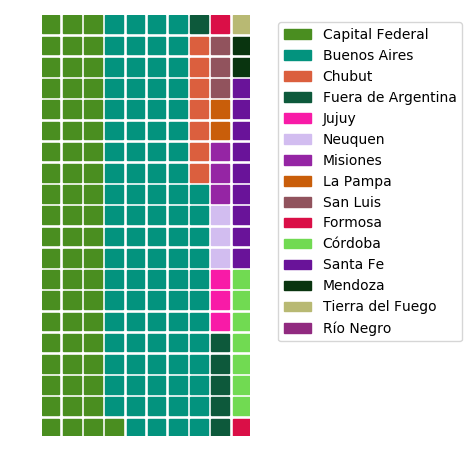
\includegraphics[scale=0.8]{datosDemograficos/infancia.png}
\end{center}
\caption{Distribución Territorial}
\label{distTerritorial}
\end{figure}

\section{Análisis de la inteligibilidad}\label{SeccionInteligibilidad}

A continuación intentaremos medir la inteligibilidad de cada una de las oraciones en base a las respuestas obtenidas en la encuesta. Para ello tomaremos la oración transcripta por los participantes y mediremos cuán lejos o cerca está de la oración original. 

Para esto utilizaremos un concepto denominado \textit{distancia de Levenshtein}. La distancia de Levenshtein consiste en calcular la menor cantidad posible de inserciones, remociones o reemplazos de caracteres que son requeridos para transformar una oración en otra. Así por ejemplo, para transformar \textit{cosa} en \textit{cal} se requieren $3$ transformaciones: reemplazar \textit{o} por \textit{a}, reemplazar \textit{s} por \textit{l} y remover la \textit{a}. Por lo tanto, la distancia de Levenshtein entre estas dos palabras es de $3$. Además, se considerará un reemplazo cualquier acento, por lo que \textit{á} y \textit{a} tendrán distancia $1$ pero no así el reemplazo de mayúsculas y minúsculas, por lo que \textit{a} y \textit{A} tendrán distancia $0$.

En la Figura \ref{resultadosGenerales} presentamos los resultados generales obtenidos sin ningún tipo de modificación a las transcripciones ingresadas por los sujetos. En el eje $x$ presentamos los grados de interpolación de inglés-castellano, que varía entre $30\%$ inglés + $70\%$ castellano (desde ahora, $30\%$ inglés) y $70\%$ inglés + $30\%$ castellano (desde ahora, $70\%$ inglés). En el eje $y$ presentamos la distancia de Levenshtein entre la oración objetivo y aquella transcripta por cada participante. Cada uno de los boxplots describe la distancia mínima obtenida y la distancia máxima (los bigotes), como así también el primer y tercer cuartil (el piso y el techo de la caja) y la mediana (línea interior que atraviesa la caja). Adicionalmente podemos observar con círculos vacíos los outliers de la muestra.


\begin{figure}
\begin{center}$
\begin{array}{lll}
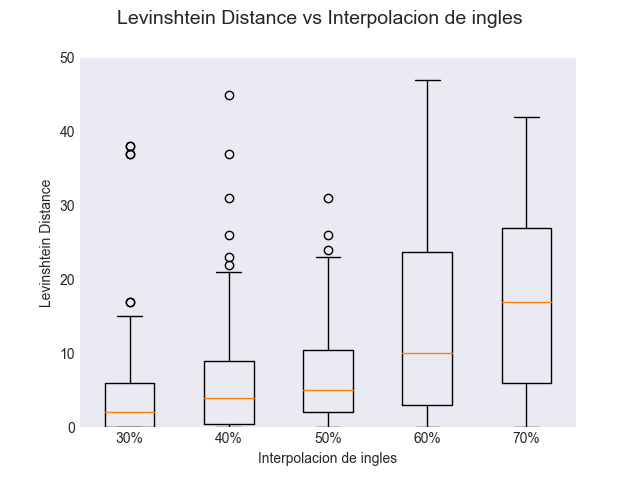
\includegraphics[trim={0 0 0 1cm},clip,width=.7\textwidth]{imagenes/plots_raw/general.png}
\end{array}$
\end{center}
\caption{Distancia de Levenshtein para distintos grados de interpolación}
\label{resultadosGenerales}
\end{figure}

Como puede observarse hasta el $50\%$ de inglés en la interpolación, la distancia entre el primer y tercer cuartil es menor a $10$ caracteres, siendo la mediana de $5$. Pasados el $60\%$ de inglés, se observa un aumento brusco en la distancia intercuartiles, la distancia entre el primer y tercer cuartil pasa a ser cercana a $20$ caracteres, y la mediana $10$ caracteres en el caso de $60\%$ inglés y $15$ en el caso del $70\%$. En las próximas secciones intentaremos encontrar una explicación intuitiva a estos números.

\section{Problemas en las transcripciones y normalización}\label{transcriptProblemsAndNorm}

Analizando detenidamente las transcripciones obtenidas podemos observar algunas fallas sistemáticas que podrían generar ruido en el análisis. Por ejemplo algunos de los participantes escribieron de manera diferente las secciones de la oración que no comprendieron. Por citar algunos ejemplos, muchos de ellos escribieron: ``...'' o simplemente omitieron la palabra, mientras que una minoría escribió cosas como ``***'', ``???'', ``\textit{blablabla}''. En los casos donde el participante no comprendió ningún segmento de la oración, es común observar expresiones como ``\textit{no entendí nada}'', ``\textit{nada}'', etc.

Por otra parte, es común la utilización innecesaria de signos de puntuación. Estos varían desde puntos finales para expresar el final de la oración hasta expresiones de confusión tales como ``(?)''. En un caso, un participante transcribió \textit{``tu estrecho posavasos'', grito la fechoría}, cuando la oración original solo decía \textit{tu estrecho portavasos gritó la fechoría}.
También pueden verse omisiones de acentos y faltas ortográficas en palabras que no presentan ambigüedades, como por ejemplo: ``\textit{grunion}'' en vez de ``\textit{gruñón}''.

Todas estas expresiones, modismos, y faltas ortográficas tienen un efecto directo y negativo sobre lo que estamos intentando medir. Así, por ejemplo, un participante que haya transcripto ``\textit{no entendí nada}'' en su respuesta devolverá una distancia de Levenshtein distinta de aquel que simplemente dejó el campo vacío, cuando en realidad estas dos respuestas expresan el mismo grado de comprensión del texto.

Con el objetivo de reducir la variabilidad en la muestra, decidimos realizar una limpieza de los datos. Intentando mantener el espíritu de las transcripciones, buscamos uniformizarlas para poder realizar un mejor análisis. Así, consideramos que si un participante escribió ``...'' en medio de una oración, su intención era la de darnos a entender que no comprendió parte de la misma. Para nuestro análisis, esto sería equivalente a no haber escrito nada. Bajo este razonamiento, consideramos que los siguientes cambios no presentan alteraciones graves en las respuestas de los participantes:

\begin{itemize}
	\item Corrección de ``ni'' por ``ñ'' en la palabra \textit{grunion}.
	\item Remoción de todos los signos de puntuación: comas, puntos, ``(?)''
	\item Reemplazo de oraciones como \textit{blabla}, \textit{no entendí} o cualquier otra expresión que indique ininteligibilidad de una palabra u oración por la cadena vacía.
	\item Corrección de acentos en palabras no ambiguas: \textit{botón}, \textit{prefirió}, \textit{recorrió}, \textit{chupetín}, \textit{riñón}, \textit{gruñón}.
\end{itemize}

Aquellas palabras que presentan ambigüedad, como \textit{concluyo}, no fueron modificadas, ya que tanto \textit{concluyó} como \textit{concluyo} son válidas. El participante podría haber interpretado la palabra con cualquiera de las dos connotaciones, cambiando el significado de la interpretación y su distancia de Levenshtein.

Confiamos en que esta limpieza nos ayudaría a disminuir el error de los resultados y también, nos permitiría interpretar de manera más intuitiva el significado de la distancia de Levenshtein en cada caso.

\section{Análisis de la inteligibilidad con los datos normalizados} \label{datosNormalizados}

Al igual que en la Sección \ref{SeccionInteligibilidad}, en la Figura \ref{generalNormalizado} presentamos los resultados de la muestra, luego de la normalización.

\begin{figure}
\begin{center}$
\begin{array}{lll}
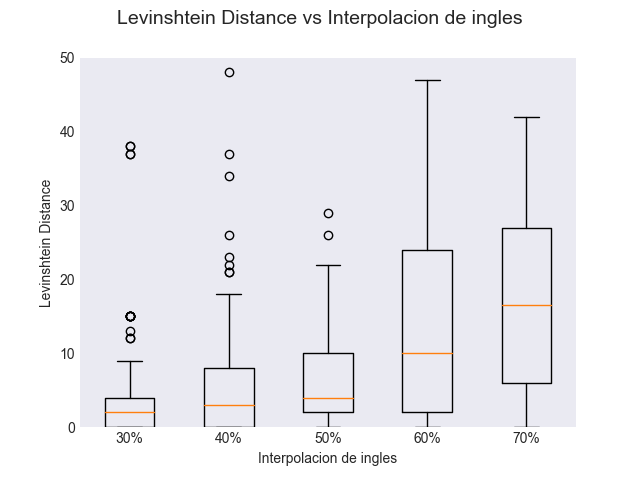
\includegraphics[trim={0 0 0 1cm},clip,width=.7\textwidth]{imagenes/plots_normalized/general.png}
\end{array}$
\end{center}
\caption{Distancia de Levenshtein para distintos grados de interpolación con datos normalizados}
\label{generalNormalizado}
\end{figure}

En esta figura podemos observar que para una interpolación de inglés de $30\%$, $96$ de los $106$ participantes obtuvieron una distancia menor a los $10$ caracteres en la transcripción del texto, mientras que los $10$ restantes, una distancia mayor a los $10$ caracteres. Podemos ver además que la distancia entre el primer y tercer cuartil es menor a $5$ caracteres con una mediana cercana a $2$ 

Para la mezcla con $40\%$ de interpolación de inglés, de un total de $67$ participantes, $57$ anotaron una distancia de Levenshtein menor a diez caracteres, $7$ una distancia entre $10$ y $30$ caracteres y $3$ una distancia mayor a $30$. La distancia intercuartil es de aproximadamente diez caracteres, con una mediana muy similar a la mezcla $30\%$ inglés.

Para la interpolación $50\%$ de inglés, de un total de $75$ participantes, $57$ lograron transcribir el audio con una distancia menor a $10$ caracteres, mientras que $14$ anotaron una distancia entre $10$ y $20$ caracteres y $4$ una distancia mayor a $20$. De manera similar que para $40\%$ la distancia intercuartil es de aproximadamente diez caracteres y la mediana de $3$ caracteres.

%Estadistica
\subsection{Análisis estadístico}

En la siguiente sección, realizaremos un análisis estadístico con el objetivo de vislumbrar cuán estadísticamente significativas son las diferencias en inteligibilidad entre los saltos de interpolación.

En primera instancia evaluamos usar el Student's two-sample t-test para este análisis. Este test pide como requerimiento que las muestras tengan una distribución normal. Para probar esto aplicamos el test de Shapiro sobre los datos normalizados.

\begin{table}
\centering
\begin{tabular}[t]{| c | c | c |}
\hline
Interpolación & p-valor & W \\
\hline
\hline
$30\%$ & 6.875e-13 & 0.5832 \\
\hline
$40\%$ & 6.875e-13 & 0.6950 \\
\hline
$50\%$ & 1.271e-06 & 0.8674 \\
\hline
$60\%$ & 2.932e-06 & 0.8694 \\
\hline
$70\%$ & 0.00215 & 0.9380\\

\hline
\end{tabular}
\caption{Test de Shapiro sobre los datos normalizados} 
\label{fig:resultadosShapiro}
\end{table}

Como puede verse en la Tabla \ref{fig:resultadosShapiro} los $5$ tests dan $p<0.01$, entonces rechazamos la hipótesis nula de normalidad, y concluimos que los datos no siguen una distribución normal. Descartamos la posibilidad de usar el Student's two-sample t-test y procedemos a utilizar el test no paramétrico Mann-Whitney-Wilcoxon, con restricciones más laxas. Este test pide como único requerimiento que las observaciones de ambos grupos sean independientes. Cabe recordar que, por diseño, nuestras observaciones cumplen con este requerimiento, ya que el sistema siempre asignaba audios con diferentes oraciones a un mismo participante, por lo que aunque contestaran más de una vez, las respuestas eran independientes entre sí.

\begin{table}
\centering
\begin{tabular}[t]{| c | c | c |}
\hline
Interpolaciones & p-valor & W \\
\hline
\hline
$30\%$ vs. $40\%$ & 0.1367 & 2041.5 \\
\hline
$40\%$ vs. $50\%$ & 0.1148 & 2132 \\
\hline
$50\%$ vs. $60\%$ & 0.0051 & 1921.5 \\
\hline
$60\%$ vs. $70\%$ & 0.0708 & 1956 \\
\hline
\end{tabular}
\caption{Resultados test no paramétrico Mann-Whitney-Wilcoxon} 
\label{tabla:Whitney}
\end{table}

Como se ve en la Tabla \ref{tabla:Whitney} la diferencia en distancia de Levinshtein entre $30\%$ y $40\%$ de interpolación de inglés no es estadísticamente significativa $(p=0.1367)$. Así tampoco lo es para el salto de $40\%$ a $50\%$ de interpolación de inglés $(p=0.1148)$. En cambio, al pasar de $50\%$ a $60\%$ la diferencia es significativa $(p=0.0051)$, lo cual se interpreta como que para este salto la inteligibilidad se deteriora más sensiblemente que para los saltos anteriores. Por último, de $60\%$ a $70\%$ la diferencia de distancias de Levinshtein es aproximadamente significativa $(p<0.1)$.

\subsection{Análisis por oración}\label{analisisPorOracion}
Tras aplicar la normalización de los datos descripta en la Sección \ref{transcriptProblemsAndNorm}, tratamos ahora de encontrar una interpretación intuitiva para las distancias de Levenshtein obtenidas. Por ejemplo, tomando la oración $8$ de las frases utilizadas en la experimentación:

\begin{itemize}
	\item ``Las acongojadas cotorras sonrieron a mi círculo''
\end{itemize}

Podemos observar las siguientes transcripciones extraídas de los $32$ resultados para esta oración:

\begin{itemize}
	\item Distancia 0: ``Las acongojadas cotorras sonrieron a mi círculo''
	\item Distancia 10: ``Las acontojadas culturas sonrieron en semicírculo''
	\item Distancia 20: ``Plaza sombreada con sombrero sonrieron en mi círculo''
	\item Distancia 30: ``sonrieron en mi círculo''
	\item Distancia 40: ``círculo''
	\item Distancia 48: ``''
\end{itemize}

Para todas las interpolaciones enunciadas previamente, los errores más comunes varían desde falta de acentos en palabras como ``concluyó'' hasta faltas de inteligibilidad en palabras con cierta complejidad fonética como ``aguileña'' o ``gruñón''. En el Apéndice \ref{transcripcionesParticipantes} listamos todas las transcripciones ingresadas por los participantes del estudio.

Como caso particular, en la oración $3$ (Figura \ref{boxplot:fig3}, $37$ respuestas), ``este enjoyado juez comprará nuestro corchete'', observamos que la mayoría de los participantes cometieron errores al transcribir la palabra ``juez'', que confundieron de manera sistemática con palabras sonoramente similares como ``fue'', ``enjoyado'', que transcribieron como ``enfollado'' o ``enrollado'', y la conjugación del verbo ``comprar'' que transcribieron como ``comprando'' o ``comprar''.

Buscando una explicación a estos errores y revisando el mapeo de fonos realizado previamente, descubrimos que el mapeo de [hh] a [g] es erróneo. Esto produjo que palabras como ``gato'' sonaran más como ``jato'' ([hh] [a] [t] [o]). Adicionalmente descubrimos que ningún fono del inglés estaba siendo mapeado al fono [x], correspondiente al grafema j en castellano. Esto produjo que cuando el sintetizador interpola entre el fono del castellano y el fono inexistente del inglés (que HTS toma como ruido blanco), el resultado fuera una mezcla entre ruido y [x]. Al ser la [x] ruido blanco (consonante fricativa), no pudimos reconocer el error en las instancias preliminares de evaluación. Esto explicaría por qué algunos participantes tuvieron problemas transcribiendo la palabra ``juez''.

Continuando con el análisis, para la interpolación de $60\%$ inglés, podemos observar un aumento notable de la variabilidad en las respuestas. Para el primero, de las $70$ respuestas obtenidas, $40$ participantes transcribieron el audio con una distancia menor a $10$ caracteres, $6$ anotaron una distancia entre $10$ y $20$ caracteres, y $24$ transcribieron el audio con distancia mayor a $20$ caracteres. Además, podemos ver en la Figura \ref{boxplot:fig3} que la distancia entre el primer y tercer cuartil es muy marcada, siendo de $20$ caracteres con una mediana igual a $10$.

Consideramos que este salto tan marcado en la distancia intercuartil puede deberse a que existen características particulares de los participantes y sus capacidades para discernir palabras, incluso cuando presentan defectos en la pronunciación del hablante. Para reforzar esa hipótesis puede verse en la figura \ref{boxplot:fig4} como en la oración $4$ para la interpolación de $70\%$ inglés, $2$ participantes de los $9$ que realizaron la transcripción, obtuvieron distancias $2$ y $6$ en sus transcripciones.

\begin{figure}
\centering
\begin{subfigure}{.5\textwidth}
  \centering
	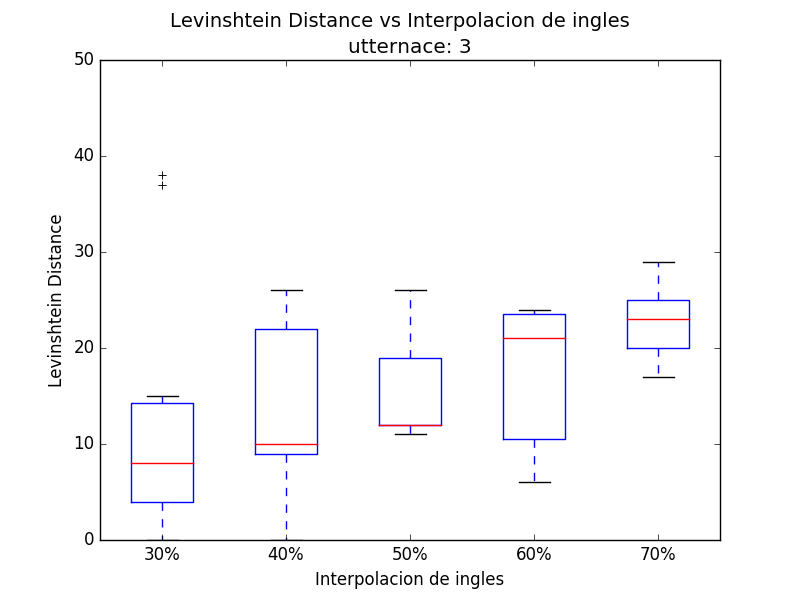
\includegraphics[trim={0 0 0 1.26cm},clip,width=1\textwidth]{imagenes/plots_normalized/3.png}
  \caption{Oración 3}
  \label{boxplot:fig3}
\end{subfigure}%
\begin{subfigure}{.5\textwidth}
  \centering
	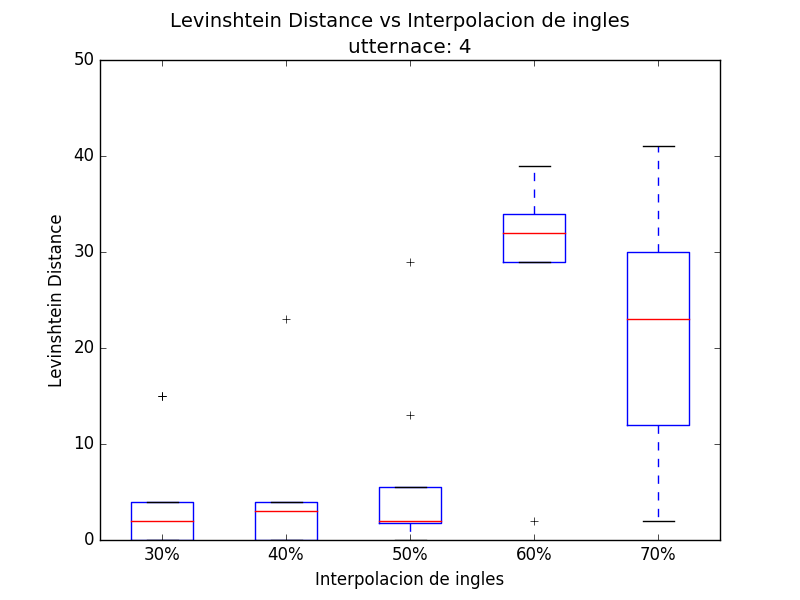
\includegraphics[trim={0 0 0 1.26cm},clip,width=1\textwidth]{imagenes/plots_normalized/4.png}
  \caption{Oración 4}
  \label{boxplot:fig4}
\end{subfigure}
\caption{Distancia de Levenshtein para distintos grados de interpolación con datos normalizados}
\label{oracionCuatro}
\end{figure}

%El segundo motivo puede deberse a que existen características particulares de las oraciones o del sintetizador generado que afectan la comprensión del audio:

Además, comparando la oración $10$ (Figura \ref{boxplot:fig10}, $32$ respuestas) ``El nudillo Argentino perdió su vaso'' con las anteriores, podemos apreciar que parecería haber características particulares en las oraciones o en el modelo generado que afectan la comprensión de los audios. Para esta oración, con $70\%$ de inglés en la interpolación, $6$ de los $8$ participantes obtuvieron una transcripción del audio con distancia menor a $15$, tanto que para la oración $3$\footnote{Tener en cuenta que ambas oraciones se encuentran afectadas por el mismo mapeo incorrecto de la [x] como fue discutido previamente}, con ese mismo grado de interpolación, todos los participantes transcribieron el audio con distancia de Levenshtein mayor a $15$. Esto parecería indicar que o bien la dificultad de las oraciones es variable o, lo que es todavía más probable, llegado cierto punto en la interpolación, algunos fonos empiezan a ``romperse'' o se alejan demasiado del fono del castellano correcto y terminan por disminuir la claridad de la voz.

\begin{figure}
\begin{center}
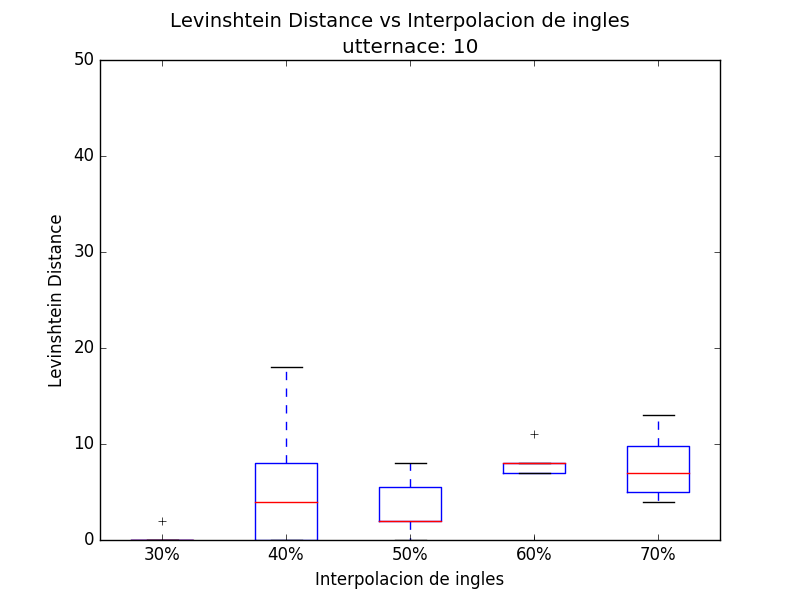
\includegraphics[trim={0 0 0 1.25cm},clip,width=.5\textwidth]{imagenes/plots_normalized/10.png}
\end{center}
\caption{Distancia de Levenshtein para distintos grados de interpolación con datos normalizados oración 10}
\label{boxplot:fig10}
\end{figure}

En esta sección analizamos distintos problemas y particularidades en las oraciones que nos permitieron descubrir errores implementativos y teorizar sobre las características del modelo generado. Pudimos ver que la comprensión de una misma oración puede variar mucho dependiendo del oyente. También pudimos ver que, incluso utilizando el mismo grado de interpolación, no todas las oraciones presentan la misma dificultad a la hora de ser interpretadas.

\section{Análisis del origen percibido}

En esta sección analizaremos los resultados de los orígenes o nacionalidades que los participantes de la encuesta atribuyeron a las voces sintetizadas. Dado que en esta instancia se le permitió a los participantes ingresar texto libre, las respuestas resultaron bastante heterogéneas. Los participantes interpretaron la consigna de distintas maneras, pudiendo encontrarse respuestas que no pueden ser atribuidas a una nacionalidad. Como ejemplo de algunas respuestas pueden encontrarse cosas como: ``Latino'', ``Anglo'', ``Robot'', ``España (sur)''. Consideramos que las respuestas de la índole ``robot'', ``es una voz artificial'', no aportan información para esta investigación. Por esta razón, en esta instancia decidimos agrupar las respuestas en cuatro conjuntos:

\begin{itemize}
	\item Hispanoparlante: ``Latino'', ``Argentino'', ``Español'', ``Uruguayo'', ``Centroamericano'', ``Boliviano'', `` Mexicano'',``Colombiano''.
	\item Angloparlante: ``Estadounidense'', ``inglés'', ``Irlandés'', ``Canadiense'', ``Anglo''.
	\item No sabe/No contesta: ``Robot'', ``no se''.
	\item Otro: ``Ruso'', ``Brasiltiño'' (sic).
\end{itemize}

Con estas agrupaciones, en la Figura \ref{analGeneral} presentamos las nacionalidades atribuidas a la voz generada para cada punto de la interpolación.

\begin{figure}
\begin{center}$
\begin{array}{lll}
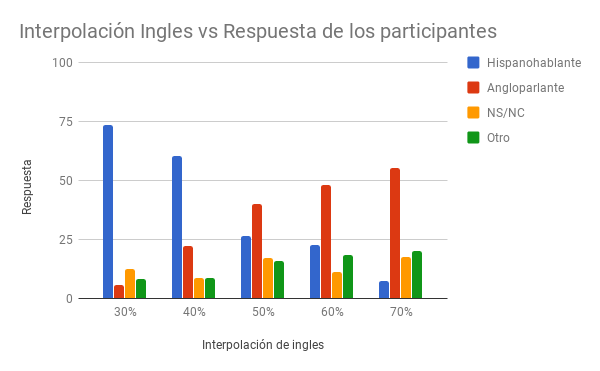
\includegraphics[trim={0 0 0 1.5cm},clip,width=.7\textwidth]{imagenes/nacionalidades/general.png}
\end{array}$
\end{center}
\caption{Interpolación inglés vs respuesta de los participantes}
\label{analGeneral}
\end{figure}

De estos resultados podemos observar que con $30\%$ de interpolación de inglés, los participantes coinciden ampliamente en que la voz puede atribuirse a una persona de habla nativa española.

En la figura pueden verse dos tendencias muy marcadas. La primera es que, a medida que aumenta el grado de interpolación de inglés, disminuye de manera lineal la cantidad de participantes que afirman que el hablante es hispánico. Dicho de otra manera, los datos parecen sugerir que con cada salto en la interpolación de inglés, la proporción de participantes que afirma que la voz pertenece a un Hispanohablante, disminuye en aproximadamente $7$ puntos perceptuales. 

Una tendencia opuesta puede notarse en los participantes que afirman que la voz es de un hablante anglosajón. A medida que aumenta el grado de interpolación de inglés, el porcentaje de atribuciones de la voz a un hablante Anglosajón aumenta aproximadamente en un $7\%$ cada vez.

Por otro lado, tanto para el conjunto ``Otro'' como para ``NS/NC'' podemos apreciar un leve aumento monótono entre los aumentos de interpolación de inglés.

%Estadistica
\subsection{Análisis estadístico}

Para darle peso estadístico a las afirmaciones realizadas en el apartado anterior, intentaremos analizar si las tendencias descendentes/ascendentes de las proporciones de sujetos que percibieron a los audios como español/inglés responden a un relación lineal con respecto al nivel de interpolación de inglés. Para eso, buscaremos ajustar un modelo lineal sobre los datos.

Como primer análisis, ajustamos un modelo lineal para la atribución del audio a una persona de habla hispana. Nuestra variable independiente será el porcentaje de interpolación de inglés en el modelo y como variable dependiente tendremos el porcentaje de sujetos que percibieron el audio como un hablante español.

\begin{figure}
\begin{center}
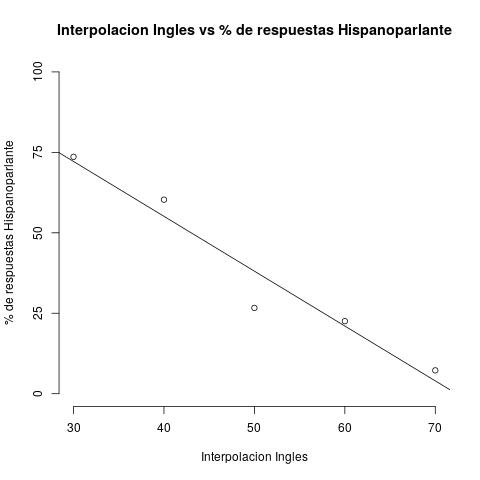
\includegraphics[trim={0 0 0 1.5cm},clip,width=.5\textwidth]{imagenes/estadistica/spanish.jpg}
\end{center}
\caption{Modelo lineal ajustado para la percepción de origen hispanoparlante}
\label{stadisticSpanish}
\end{figure}

Como puede verse en la Figura \ref{stadisticSpanish} el modelo lineal ajustado explica satisfactoriamente los datos, con un nivel elevado de significancia estadística $(p<0.01)$.

Como segundo análisis, ajustamos otro modelo lineal para la percepción de atribuciones de la nacionalidad a una persona angloparlante. En este caso la variable independiente será nuevamente el grado de interpolación de inglés y como variable dependiente tendremos el porcentaje de sujetos que percibieron el audio como un hablante inglés.

\begin{figure}
\begin{center}
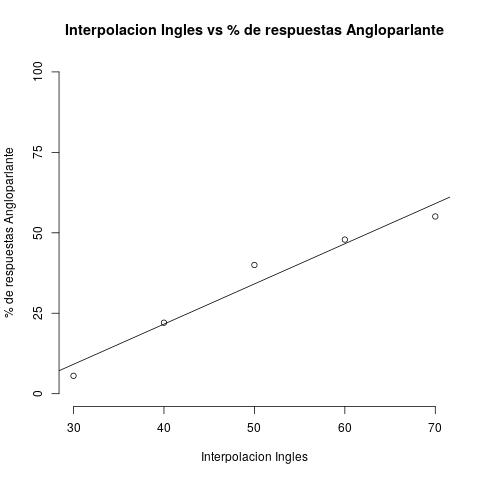
\includegraphics[trim={0 0 0 1.5cm},clip,width=.5\textwidth]{imagenes/estadistica/english.jpg}
\end{center}
\caption{Modelo lineal ajustado para la percepción de origen angloparlante}
\label{stadisticEnglish}
\end{figure}

En la Figura \ref{stadisticEnglish} puede verse que el modelo lineal ajustado explica satisfactoriamente los datos, con un nivel elevado de significancia estadística $(p<0.05)$.

De esto podemos concluir que existe evidencia estadística que indica que aumentar el grado de interpolación resulta en más participantes reconociéndolo como una persona de habla inglesa y no como un hablante oriundo de un país de habla hispana.

\subsection{Análisis por oración}

Observando las oraciones una por una, podemos ver algunas discrepancias con los resultados generales. Por ejemplo, en la oración $9$ (``Ese gruñón perro prometió a esos cuñados''), con un $40\%$ de interpolación de inglés, el $60\%$ de los participantes ($16$ de los $30$ que contestaron la encuesta) considera que la voz pertenece a un hablante de habla anglosajona, siendo que en los resultados generales, para ese mismo grado de interpolación, menos del $25\%$ de los participantes lo afirmaban.

\begin{figure}
\begin{center}$
\begin{array}{lll}
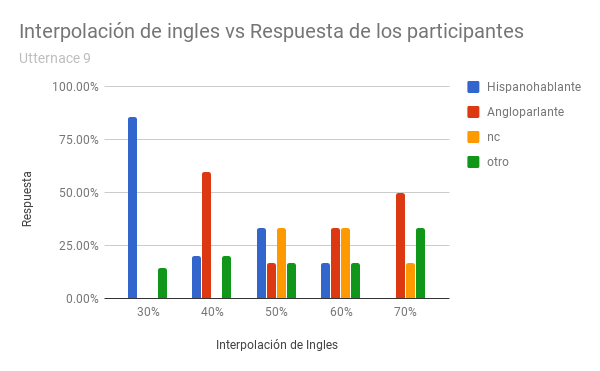
\includegraphics[trim={0 0 0 2.3cm},clip,width=.7\textwidth]{imagenes/nacionalidades/9.png}
\end{array}$
\end{center}
\caption{Interpolación de inglés vs Respuestas de los participantes, oración 9}
\label{tresNueve}
\end{figure}

Aunque este fenómeno puede deberse a la cantidad reducida de datos con los que trabajamos, no debe descartarse la posibilidad de que esta gran diferencia entre los resultados se pueda atribuir a las características particulares de cada oración. En particular la oración $9$ contiene una [\textipa{r}] (\textit{perro}) que resulta muy notoria al pronunciarse con una intensidad menor a la esperada (más similar a una [\textipa{R}] (\textit{pero})) y puede ser atribuida, entre otras causas, a un hablante Anglosajón con dificultades en la dicción de fonos extranjeros.
%perro vibrante múltiple alveolar sonora

Bajo esta suposición buscamos en qué otras oraciones se presenta este fono:

\begin{itemize}
\item Oración $1$: ``Mi montaña aguileña recorrió la esquina'' 
\item Oración $6$: ``Su profundo riñón apoyó a Julio''
\item Oración $7$: ``El frío churrasco oyó lo de Polonia''
\item Oración $8$: ``Las acongojadas cotorras sonrieron a mi círculo''
\end{itemize}

En la Figura \ref{unoSeis} podemos observar que las oraciones $1$ y $7$ (con $37$ respuestas cada una) también tienen una marcada diferenciación respecto a los resultados generales. En particular estas dos oraciones no describen el comportamiento monótono observado previamente. 

\begin{figure}
\centering
\begin{subfigure}{.5\textwidth}
  \centering
	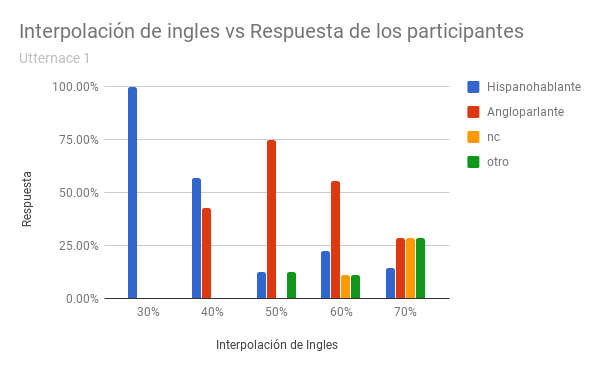
\includegraphics[trim={0 0 0 2.5cm},clip,width=1\textwidth]{imagenes/nacionalidades/1.png}
  \caption{Oración 1}
\end{subfigure}%
\begin{subfigure}{.5\textwidth}
  \centering
	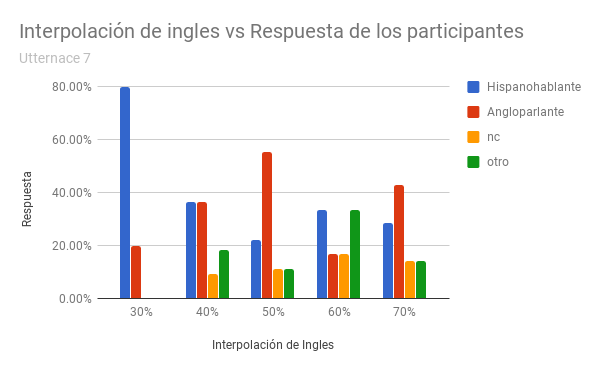
\includegraphics[trim={0 0 0 2.5cm},clip,width=1\textwidth]{imagenes/nacionalidades/7.png}
  \caption{Oración 7}
\end{subfigure}
\caption{Interpolación de inglés vs respuesta de los participantes}
\label{unoSeis}
\end{figure}


Por otro lado en la Figura \ref{sieteOcho} mostramos los resultados obtenidos para las oraciones $6$ ($41$ respuestas) y $8$ ($30$ respuestas). En estos casos no pueden observarse diferencias notorias al compararlos contra los resultados generales. Ambas oraciones presentan el mismo comportamiento monótono, que al tener una menor cantidad de datos, se observa de manera más difusa.


\begin{figure}
\centering
\begin{subfigure}{.5\textwidth}
  \centering
	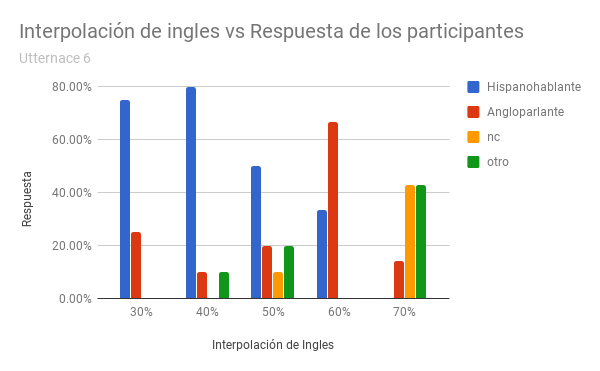
\includegraphics[trim={0 0 0 2.5cm},clip,width=1\textwidth]{imagenes/nacionalidades/6.png}
  \caption{Oración 6}
\end{subfigure}%
\begin{subfigure}{.5\textwidth}
  \centering
	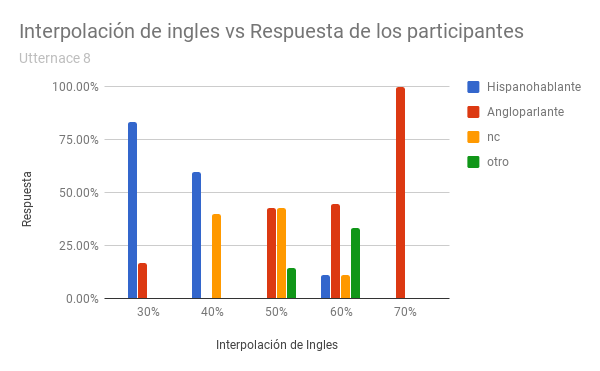
\includegraphics[trim={0 0 0 2.5cm},clip,width=1\textwidth]{imagenes/nacionalidades/8.png}
  \caption{Oración 8}
\end{subfigure}
\caption{Interpolación de inglés vs respuesta de los participantes}
\label{sieteOcho}
\end{figure}

Hasta ahora analizamos los dos ejes de nuestra hipótesis por separado (por un lado, inteligibilidad, por otro, nacionalidad atribuida a la voz). En la última sección de la investigación buscaremos sacar conclusiones al componer ambos ejes en un mismo análisis.

\section{Resultados generales de la experimentación}

En la Figura \ref{resultadosGeneralesNacVsPlot} presentamos los resultados comparando las distancias de Levenshtein con los porcentajes de participantes que determinaron que el hablante fuera anglosajón. Al igual que en el Apartado \ref{SeccionInteligibilidad}, en el eje $x$ presentamos los grados de interpolación de inglés, yendo desde $30\%$ hasta $70\%$. El eje $y$ del lado izquierdo representa la distancia de Levenshtein  entre la oración objetivo y aquella transcripta por cada participante. Cada uno de los boxplots describe la distancia mínima obtenida y la distancia máxima (los bigotes), como así también el primer y tercer cuartil (el piso y el techo de la caja) y la mediana (línea interior que atraviesa la caja). Adicionalmente podemos observar con círculos vacíos los outliers de la muestra. En el eje $y$ del lado derecho, presentamos el porcentaje de participantes que atribuyeron la voz a un hablante anglosajón indicado mediante puntos verdes en el gráfico. 

\begin{figure}
\begin{center}$
\begin{array}{lll}
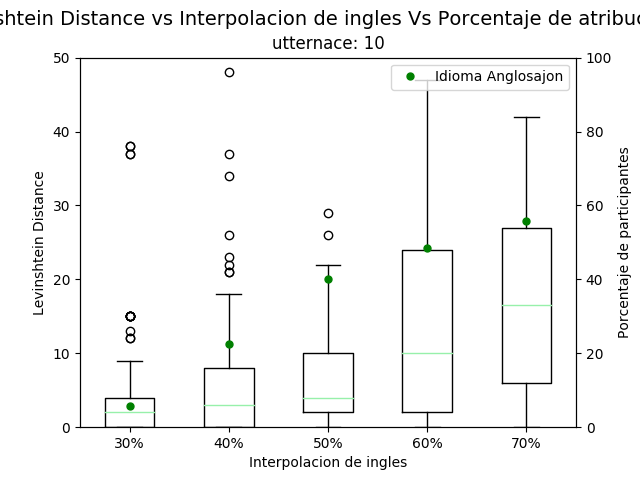
\includegraphics[trim={0 0 0 1.3cm},clip,width=.7\textwidth]{imagenes/nacVsPlot/general.png}
\end{array}$
\end{center}
\caption{Distancia de Levenshtein vs distintos grados de interpolación vs Porcentaje de participantes que reportaron hablante anglosajón}
\label{resultadosGeneralesNacVsPlot}
\end{figure}

En esta figura podemos apreciar que para cada aumento en el grado de interpolación de inglés, tanto el porcentaje de participantes que considera la voz como un hablante anglosajón como la mediana de la distancia de Levenshtein crecen de manera monótona. Comenzando con un $5\%$ de participantes afirmando que la voz anglosajona y una mediana de la distancia de Levenshtein de $3$ para una interpolación de $30\%$ inglés, y llegando hasta $55\%$ de participantes afirmando que la voz pertenecía a un hablante anglosajón y una mediana de aproximadamente $18$ caracteres para la interpolación de $70\%$ inglés.

En base a estos resultados podemos afirmar que la hipótesis original tiene cierto grado de validez experimental: la interpolación de HMMs descripta en esta tesis es un método válido para generar voces que pueden ser identificadas con un nativo anglosajón hablando castellano. Sin embargo esto viene con un costo asociado: la claridad de las oraciones disminuirá a medida que se aumenta el grado de interpolación del modelo de inglés.
